\documentclass[
    hyperref = {hidelinks, linkcolor = black},
    xcolor = {dvipsnames},
    10pt
    aspectration = 169
]{beamer}

% \usepackage{atveryend}
\usepackage{varwidth}
\usepackage{bookmark}
\usepackage{microtype}
\usepackage[numbers]{natbib}

\usepackage{graphicx}
\usepackage{caption}
\captionsetup[figure]{labelformat = empty}
\usepackage{subcaption}
\captionsetup[subfigure]{labelformat = empty}

\usepackage{tikz}
\usetikzlibrary{
    % spy,
    arrows,
    arrows.meta,
    automata,
    calc,
    % decorations.markings,
    fit,
    graphs,
    hobby,
    intersections,
    % patterns,
    positioning,
    quotes,
    shapes.geometric,
    shapes.misc
}

% AMSMATH IS PICKY ABOUT BEING LOADED BEFORE SOME OTHER PACKAGES
\usepackage{amsmath}

% THEOREMS, DEFINITIONS, EXAMPLES, ETC.
\usepackage{amsthm}
\usepackage[theorems, skins]{tcolorbox}

\usepackage{mathtools}
\usepackage{fourier-otf}
\usepackage{stmaryrd}

% LISTS
\usepackage[inline]{enumitem}

\setlist[itemize]{
    leftmargin = 15pt,
    itemsep = 1ex,
    % parsep = 0.25ex,
    topsep = 1ex,
    label = \raisebox{0.33ex}{\scalebox{0.75}{$\blacktriangleright$}}
}

\setlist[enumerate]{
    leftmargin = 15pt,
    itemsep = 1ex,
    % parsep = 0.25ex,
    topsep = 1ex,
    label = (\arabic*)
}


% TABLES
\usepackage{booktabs}
\usepackage{makecell}


% BEAMER JUNK
\useoutertheme[
    numbering = fraction,
    progressbar = frametitle
]{metropolis}

\useinnertheme[
    sectionpage = progressbar,
    subsectionpage = progressbar
]{metropolis}

\usefonttheme[titleformat title = regular]{metropolis}
\usefonttheme[onlymath]{serif}
\setsansfont[BoldFont={Fira Sans SemiBold}]{Fira Sans Book}
\setbeamerfont{page number in head/foot}{size = \tiny}

\usecolortheme{spruce}
% \usecolortheme{spruce}
% \usefonttheme{serif}

\setbeamersize{
    text margin left = 15pt,
    text margin right = 15pt
}

\defbeamertemplate{section page}{myprogressbar}{
    \centering
    \begin{minipage}{\textwidth}
        \raggedright
        \usebeamercolor[fg]{section title}
        \usebeamerfont{section title}
        \insertsectionhead\\[-1ex]
        \usebeamertemplate*{progress bar in section page}
        \mbox{}\\
        \par
    \end{minipage}
    \par
    \vspace{\baselineskip}
}

\defbeamertemplate{subsection page}{myprogressbar}{
    \centering
    \begin{minipage}{\textwidth}
        \raggedright
        \usebeamercolor[fg]{section title}
        \usebeamerfont{section title}
        \insertsectionhead\\[-1ex]
        \usebeamertemplate*{progress bar in section page}
        \mbox{}\\
        \par
        \ifx\insertsubsectionhead\@empty\else%
        \usebeamercolor[fg]{subsection title}%
        \usebeamerfont{subtitle}%
        \tableofcontents[sectionstyle = hide/hide, subsectionstyle = show/shaded/hide]
        \fi
    \end{minipage}
    \par
    \vspace{\baselineskip}
}

\setbeamertemplate{section page}[myprogressbar]
\setbeamertemplate{subsection page}[myprogressbar]
% \setbeamertemplate{background}[grid]
% \setbeameroption{show notes}

% FONTS
\newcommand{\tu}[1]{\textup{#1}}
\newcommand{\tb}[1]{\textbf{#1}}
\newcommand{\tn}[1]{\tu{#1}}
\newcommand{\ts}[1]{\textsf{#1}}
\newcommand{\tsc}[1]{\textsc{#1}}
\newcommand{\bb}[1]{\ensuremath{\mathbb{#1}}}
\newcommand{\ms}[1]{\ensuremath{\mathsf{#1}}}
\newcommand{\mc}[1]{\ensuremath{\mathcal{#1}}}
\newcommand{\mb}[1]{\ensuremath{\mathbf{#1}}}
\renewcommand{\vec}[1]{\ensuremath{\bm{#1}}}
\newcommand{\mf}[1]{\ensuremath{\mathfrak{#1}}}
\newcommand{\mt}[1]{\ensuremath{\mathtt{#1}}}
\newcommand{\msc}[1]{\ensuremath{\mathscr{#1}}}


% PAIRED DELIMITERS
\DeclarePairedDelimiter\set{\lbrace}{\rbrace}
\DeclarePairedDelimiter\sem{\llbracket}{\rrbracket}
\DeclarePairedDelimiter\paren{(}{)}
\DeclarePairedDelimiter\tup{\langle}{\rangle}
\DeclarePairedDelimiter\seq{(}{)}
\DeclarePairedDelimiter\card{\lvert}{\rvert}
\DeclarePairedDelimiter\brak{[}{]}
% \DeclarePairedDelimiter\numsem{\llangle}{\rrangle}
\DeclarePairedDelimiter\floor{\lfloor}{\rfloor}

% PAST-DISCOUNTING STUFF
% \newcommand{\last}[1]{\ms{last}\paren*{#1}}
\newcommand{\cond}[1]{\tu{Cnd}\paren*{#1}}
\newcommand{\icond}[2]{\tu{Cnd}^\top_{#1,\flat}\paren*{#2}}
\newcommand{\scond}[2]{\tu{Cnd}^\top_{#1,\sharp}\paren*{#2}}
\newcommand{\val}[3]{\tu{Val}_{#2}\paren*{#1, #3}}
\newcommand{\pval}[4]{\tu{Val}^{#4}_{#2}\paren*{#1, #3}}
\newcommand{\Path}[1]{\tu{Path}\paren*{#1}}
\newcommand{\Traj}[1]{\tu{Traj}\paren*{#1}}
\newcommand{\xPath}[2]{\tu{Path}_{#2}\paren*{#1}}
\newcommand{\xTraj}[2]{\tu{Traj}_{#2}\paren*{#1}}
\newcommand{\sPath}{\tu{Path}}
\newcommand{\sTraj}{\tu{Traj}}
\newcommand{\sbsq}[3]{#1{\scriptstyle\brak*{#2, #3}}}
\DeclareMathOperator*{\limopt}{\tu{lim}~\tu{opt}}
\newcommand{\shortflat}{\scalebox{1}[.66]{$\flat$}}
\newcommand{\uPD}{\ms{P}^\sharp_\gamma}
\newcommand{\lPD}{\ms{P}^{\shortflat}_\gamma}
\newcommand{\PD}{\ms{P}^\natural_\gamma}
\newcommand{\transpose}[1]{{#1}^{\intercal}}


% STANDARDIZED ABBREVIATIONS
\newcommand{\eg}{\emph{e.g.}}
\newcommand{\cf}{\emph{cf.}}
\newcommand{\ie}{\emph{i.e.}}
\newcommand{\etc}{\emph{etc.}}

% CONVENIENCE
\newcommand{\w}{\ensuremath{\omega}}
\newcommand{\nth}[1]{{#1}^{\tu{th}}}
\newcommand{\bigast}{\mathop{\scalebox{1.75}{\raisebox{-0.2ex}{$\ast$}}}}
\newcommand{\largediamond}{\mathop{\scalebox{1.75}{\raisebox{-0.2ex}{$\diamond$}}}}
\newcommand{\Emph}[1]{\emph{\textrm{#1}}}

% COMPLEXITY CLASSES
\newcommand{\dspace}[1]{\textrm{DSPACE}\ensuremath{\paren*{#1}}}

\tikzset{
    every picture/.style = {
        > = Stealth,
        thick,
        initial text =
    },
    loop/.append style = {
        looseness = 5,
        min distance = 0.5cm
    },
    loop above/.append style = {out = 110, in = 70 },
    loop below/.append style = {out = 290, in = 250},
    loop left/.append  style = {out = 200, in = 160},
    loop right/.append style = {out = 20,  in = 340},
    every state/.style = {
        inner sep = 2pt,
        outer sep = 0pt,
        minimum size = 15pt
    },
    every node/.style = {
        inner sep = 1pt,
        outer sep = 2pt,
        minimum size = 0pt,
        fill = white,
        align = center
    },
    graphs/edge quotes = {
        inner sep = 1pt,
        outer sep = 2pt,
        fill = white
    },
    dots/.style args = {#1per #2}{%
        line cap=round,
        dash pattern=on 0 off #2/#1
    }
}

% COLORS
\newcommand{\red}[1]{{\color{red}#1}}
\newcommand{\blue}[1]{{\color{blue}#1}}
\newcommand{\teal}[1]{{\color{teal}#1}}
\newcommand{\violet}[1]{{\color{Violet}#1}}
\newcommand{\purple}[1]{{\color{purple}#1}}
\newcommand{\grey}[1]{{\color{gray}#1}}
\newcommand{\cyan}[1]{{\color{cyan}#1}}
\newcommand{\green}[1]{{\color{Green}#1}}
\newcommand{\magenta}[1]{{\color{magenta}#1}}
\newcommand{\rblue}[1]{{\color{RoyalBlue}#1}}

% THEOREM-LIKE ENVIRONMENTS
\DeclareTcbTheorem[no counter]{theorem}{Theorem}{
    enhanced,
    frame empty,
    % interior empty,
    colback = Cerulean!5!white,
    colframe = Cerulean!50!white,
    coltitle = black,
    fonttitle = \footnotesize\bfseries,
    colbacktitle = Cerulean!25!white,
    borderline = {0.5mm}{0mm}{Cerulean!50},
    attach boxed title to top left = {
        xshift = 5pt,
        yshift = -5pt
    },
    boxed title style = {boxrule = 1pt},
    varwidth boxed title,
    label separator = {:},
    separator sign colon,
    fontupper = \footnotesize
}{thm}

% \DeclareTcbTheorem[no counter]{definition}{Definition}{
%     enhanced,
%     frame empty,
%     interior empty,
%     colframe = MidnightBlue!50!white,
%     coltitle = black,
%     fonttitle = \bfseries,
%     colbacktitle = MidnightBlue!15!white,
%     borderline = {0.5mm}{0mm}{MidnightBlue!50},
%     attach boxed title to top left = {
%         xshift = 5pt,
%         yshift = -5pt
%     },
%     boxed title style = {boxrule = 1pt},
%     varwidth boxed title,
%     label separator = {:},
%     separator sign colon,
%     fontupper = \footnotesize
% }{def}

\DeclareTcbTheorem[no counter]{corollary}{Corollary}{
    enhanced,
    frame empty,
    % interior empty,
    colback = Apricot!5!white,
    colframe = Apricot!50!white,
    coltitle = black,
    fonttitle = \footnotesize\bfseries,
    colbacktitle = Apricot!25!white,
    borderline = {0.5mm}{0mm}{Apricot!75},
    attach boxed title to top left = {
        xshift = 5pt,
        yshift = -5pt
    },
    boxed title style = {boxrule = 1pt},
    varwidth boxed title,
    label separator = {:},
    separator sign colon,
    fontupper = \footnotesize
}{cor}


% \tikzexternalize[prefix = figures/]
% % INJECTING CODE BEFORE/AFTER SPECIFIC ENVIRONMENTS
% \BeforeBeginEnvironment{definition}{\tikzexternaldisable}
% \AfterEndEnvironment{definition}{\tikzexternalenable}
% \BeforeBeginEnvironment{theorem}{\tikzexternaldisable}
% \AfterEndEnvironment{theorem}{\tikzexternalenable}
% \BeforeBeginEnvironment{corollary}{\tikzexternaldisable}
% \AfterEndEnvironment{corollary}{\tikzexternalenable}


\renewcommand{\thefootnote}{\raisebox{1ex}{\tiny\fnsymbol{footnote}}}

\usepackage{bm}

\title{Regular Reinforcement Learning}
\author{\teal{Taylor Dohmen}, Mateo Perez, Fabio Somenzi, \& Ashutosh Trivedi}
\institute{University of Colorado Boulder}

\begin{document}

    \begin{frame}
        \maketitle
    \end{frame}


    % \begin{frame}
    %     \begin{itemize}
    %         \item Motivate choice of regular languages.
    %         \item talk about idea of symbolic motivation.
    %     \end{itemize}
    
    % \end{frame}

    \begin{frame}
        \begin{figure}
            \centering
            \includegraphics[width = 0.75\linewidth]{~/Documents/projects/DissertationDefense/agent-environment.png}
        \end{figure}
    \end{frame}
    

    % \section{Regular Markov Decision Processes}

    \begin{frame}{Inspiration --- Regular Model Checking (RMC)}

        \footnotesize Infinite (non-stochastic) systems are modeled such that
        \begin{itemize}
            \item states are expressed with regular languages,
            \item state transitions are expressed as rational transductions.
        \end{itemize}

        % \begin{overprint}
            
            % \onslide<1>
            % \begin{center}
            %     \begin{tikzpicture}
            %         % \draw[step = 1cm, lightgray, very thin] (-2, -2) grid (7, 5);
            %        \path[draw, use Hobby shortcut, closed = true] (0, 0) .. (.5, 1) .. (-0.25, 3) .. (.3, 4) .. (-1, 2) .. (-1, .5);
    
            %     %    \path[draw, use Hobby shortcut, closed = true] (5, 0) .. (5.5, 1) .. (6.25, 3) .. (5.3, 4) .. (4, 2) .. (4, .5);
    
            %        \node at (-0.5, 2) {$L$};
            %        \node[draw = none] at (5, 2) {}; %{$\theta(L)$};
    
            %        \node[draw = none] at (-2, 2) {\scriptsize \teal{regular} \\ \scriptsize \teal{language}};
            %        \node[draw = none] at (7, 2) {}; %{\scriptsize \teal{regular} \\ \scriptsize \teal{language}};
            %     %    \path[->] (0, 2) edge node[label = {\scriptsize \teal{rational} \\ \scriptsize \teal{transduction}}] {$\theta$} (4, 2);
            %    \end{tikzpicture}
            % \end{center}

            % \onslide<2>
            % \begin{center}
            %     \begin{tikzpicture}
            %         % \draw[step = 1cm, lightgray, very thin] (-2, -2) grid (7, 5);
            %        \path[draw, use Hobby shortcut, closed = true] (0, 0) .. (.5, 1) .. (-0.25, 3) .. (.3, 4) .. (-1, 2) .. (-1, .5);
    
            %        \path[draw, use Hobby shortcut, closed = true] (5, 0) .. (5.5, 1) .. (6.25, 3) .. (5.3, 4) .. (4, 2) .. (4, .5);
    
            %        \node at (-0.5, 2) {$L$};
            %        \node at (5, 2) {$\theta(L)$};
    
            %        \node at (-2, 2) {\scriptsize \teal{regular} \\ \scriptsize \teal{language}};
            %     %    \node at (7, 2) {\scriptsize \teal{regular} \\ \scriptsize \teal{language}};
            %        \path[->] (0, 2) edge node[label = {\scriptsize \teal{rational} \\ \scriptsize \teal{transduction}}] {$\theta$} (4, 2);
            %    \end{tikzpicture}
            % \end{center}

            % \onslide<1>
            \begin{center}
                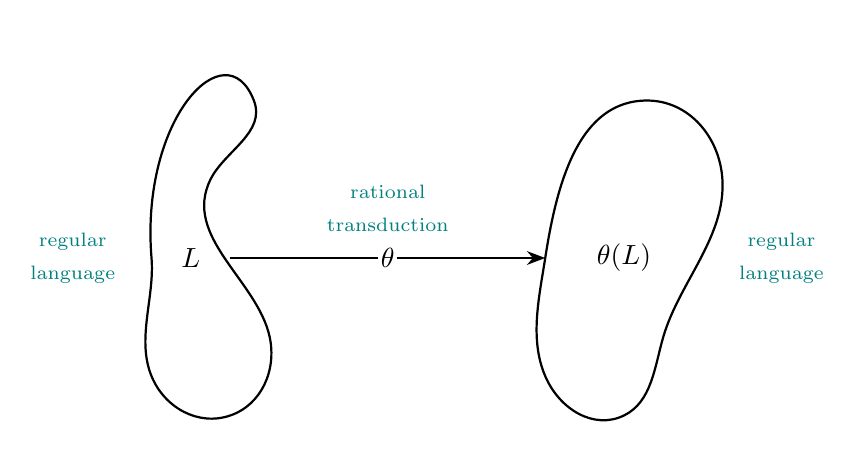
\begin{tikzpicture}
                    % \draw[step = 1cm, lightgray, very thin] (-2, -2) grid (7, 5);
                   \path[draw, use Hobby shortcut, closed = true] (0, 0) .. (.5, 1) .. (-0.25, 3) .. (.3, 4) .. (-1, 2) .. (-1, .5);
    
                   \path[draw, use Hobby shortcut, closed = true] (5, 0) .. (5.5, 1) .. (6.25, 3) .. (5.3, 4) .. (4, 2) .. (4, .5);
    
                   \node at (-0.5, 2) {$L$};
                   \node at (5, 2) {$\theta(L)$};
    
                   \node at (-2, 2) {\scriptsize \teal{regular} \\ \scriptsize \teal{language}};
                   \node at (7, 2) {\scriptsize \teal{regular} \\ \scriptsize \teal{language}};
                   \path[->] (0, 2) edge node[label = {\scriptsize \teal{rational} \\ \scriptsize \teal{transduction}}] {$\theta$} (4, 2);
               \end{tikzpicture}
            \end{center}

        % \end{overprint}
        
    \end{frame}

    \begin{frame}{An RMC Example --- Token Passing}

        \vspace{2ex}

        \begin{columns}
            \begin{column}{0.5\linewidth}
                % \begin{center}
                    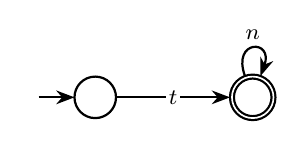
\begin{tikzpicture}[font = \footnotesize]
                        \node[state, initial] (0) {};
                        \node[state, accepting] (1) at (2, 0) {};
                        \path[->] (0) edge node {$t$} (1);
                        \path[->] (1) edge[loop above] node {$n$} (1);
                    \end{tikzpicture}
                % \end{center}

                \teal{\footnotesize
                    automaton for initial language $I = t n^*$
                }
            \end{column}
            \begin{column}{0.5\linewidth}
                % \begin{center}
                    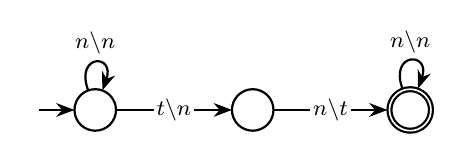
\begin{tikzpicture}[font = \footnotesize]
                        \node[state, initial] (0) {};
                        \node[state] (1) at (2, 0) {};
                        \node[state, accepting] (2) at (4, 0) {};
                        \path[->] (0) edge[loop above] node {$n \backslash n$} (0);
                        \path[->] (0) edge node {$t \backslash n$} (1);
                        \path[->] (1) edge node {$n \backslash t$} (2);
                        \path[->] (2) edge[loop above] node {$n \backslash n$} (2);
                    \end{tikzpicture}
                % \end{center}

                \teal{\footnotesize transducer $T$ passes token 1 index right}
            \end{column}
        \end{columns}

        \vspace{3ex}

        \begin{center}
            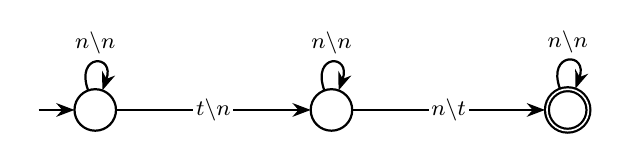
\begin{tikzpicture}[font = \footnotesize]
                \node[state, initial] (0) {};
                \node[state] (1) at (3, 0) {};
                \node[state, accepting] (2) at (6, 0) {};
                \path[->] (0) edge[loop above] node {$n \backslash n$} (0);
                \path[->] (0) edge node {$t \backslash n$} (1);
                \path[->] (1) edge[loop above] node {$n \backslash n$} (1);
                \path[->] (1) edge node {$n \backslash t$} (2);
                \path[->] (2) edge[loop above] node {$n \backslash n$} (2);
            \end{tikzpicture}

            \teal{\footnotesize transducer $T^+$ moves the token rightwards by an arbitrary number of positions}

            \vspace{2ex}

            \tcbox[colback = white, colframe = teal]{
                $\displaystyle T^+(I) = n^* t n^*$
            }
            \footnotesize Reachable Language
        \end{center}
    \end{frame}

    \begin{frame}{Regular Markov Decision Processes (RMDPs)}

        % \footnotesize Infinite-state Markov decision processes 
        % \begin{itemize}
        %     \item states are represented as regular languages,
        %     \item transitions are represented as rational transductions. 
        % \end{itemize}
        
        \begin{center}
            \vspace{-4ex}
            % \resizebox{!}{0.75\textheight}{
                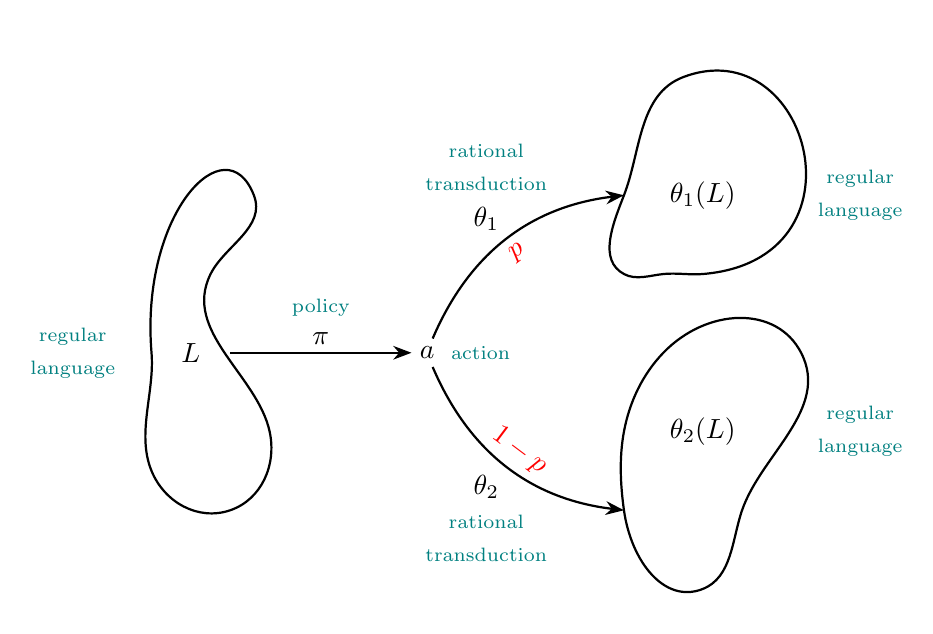
\begin{tikzpicture}
                    % \draw[step = 1cm, lightgray, very thin] (-2, -5) grid (7, 5);
                    \path[draw, use Hobby shortcut, closed = true] (-1, 0) .. (-0.5, 1) .. (-1.25, 3) .. (-0.7, 4) .. (-2, 2) .. (-2, 0.5);
    
                    \path[draw, use Hobby shortcut, closed = true] (5, -1) .. (5.5, 0) .. (6.25, 2) .. (4.5, 2) .. (4, 1) .. (4, 0);
    
                    \path[draw, use Hobby shortcut, closed = true] (4.5, 3) .. (5, 3) .. (4.75, 5.5) .. (4, 4) .. (4, 3);
    
                    \node[label = {0:{\scriptsize \teal{action}}}] (a) at (1.5, 2) {$a$};
    
                    \node at (-1.5, 2) {$L$};
                    \node at (5, 1) {$\theta_2(L)$};
                    \node at (5, 4) {$\theta_1(L)$};
    
                    \node at (-3, 2) {\scriptsize \teal{regular} \\ \scriptsize \teal{language}};
                    \node at (7, 1) {\scriptsize \teal{regular} \\ \scriptsize \teal{language}};
                    \node at (7, 4) {\scriptsize \teal{regular} \\ \scriptsize \teal{language}};
                    \path[->] (-1, 2) edge node[above, fill = none, label = {\scriptsize \teal{policy}}] {$\pi$} (a);
    
                    \path[->] (a) edge[bend right] node[below left, fill = none, label = {270:\scriptsize \teal{rational} \\ \scriptsize \teal{transduction}}] {$\theta_2$} node[above, sloped] {$\red{1-p}$} (4, 0);
                    \path[->] (a) edge[bend left] node[above left, fill = none, label = {\scriptsize \teal{rational} \\ \scriptsize \teal{transduction}}] {$\theta_1$} node[below, sloped] {$\red{p}$} (4, 4);
                \end{tikzpicture}
            % }
        \end{center}
    \end{frame}

    \begin{frame}{RMDP Example --- A Variation on Token Passing}
        \footnotesize

        3 actions are available to the agent:
        % {\scriptsize
            \begin{enumerate}[label = ($\alph*$)]
                \item
                    Each odd-index with a token passes it right.\\
                    Each even-index with a token passes it right \& generates itself a new token.
                \item
                    Each even-index with a token passes it right.\\
                    Each odd-index with a token passes it right \& generates itself a new token.
                \item
                    Mimics action ($a$) with probability $p$ and mimics action ($b$) with probability $1-p$
            \end{enumerate}
        % }

        \begin{equation*}
            \tn{reward at } L = \begin{cases}
                0 &\tn{if } L \subseteq n^* t n^* \\
                -1 &\tn{otherwise}
            \end{cases}
        \end{equation*}

        \begin{figure}
            \centering
            \begin{subfigure}{0.5\linewidth}
                \centering
                \resizebox{0.75\linewidth}{!}{
                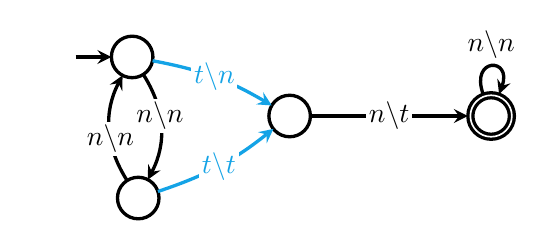
\begin{tikzpicture}[very thick, > = stealth]
                    \node (0) {};
                    \node[state, initial] (1)[above right = 1.5cm and 1cm of 0] {};
                    \node[state] (2)[right = 1cm of 0] {};
                    \node[state] (3)[above right = 0.75cm and 3cm of 0] {};
                    \node[state, accepting] (4)[right = 2cm of 3] {};
        
                    \path[->] (1) edge[bend left] node[pos = 0.4] {$n \backslash n$} (2);
                    \path[->] (2) edge[bend left] node[pos = 0.4] {$n \backslash n$} (1);
                    \path[->, color = Cerulean] (1) edge[bend left = 10] node {$t \backslash n$} (3);
                    \path[->, color = Cerulean] (2) edge[bend right = 10] node {$t \backslash t$} (3);
                    \path[->] (3) edge node {$n \backslash t$} (4);
                    \path[->] (4) edge[loop above] node {$n \backslash n$} (4);
                \end{tikzpicture}
                }
                \vspace{-3ex}
                \caption{\hspace{2cm} \scriptsize \color{teal} transducer $T_{a}$}
            \end{subfigure}%
            \begin{subfigure}{0.5\linewidth}
                \centering
                \resizebox{0.75\linewidth}{!}{
                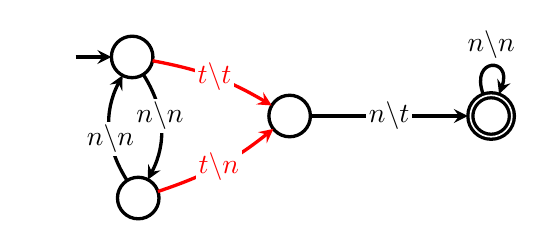
\begin{tikzpicture}[very thick, > = stealth]
                    \node (0) {};
                    \node[state, initial] (1)[above right = 1.5cm and 1cm of 0] {};
                    \node[state] (2)[right = 1cm of 0] {};
                    \node[state] (3)[above right = 0.75cm and 3cm of 0] {};
                    \node[state, accepting] (4)[right = 2cm of 3] {};
        
                    \path[->] (1) edge[bend left] node[pos = 0.4] {$n \backslash n$} (2);
                    \path[->] (2) edge[bend left] node[pos = 0.4] {$n \backslash n$} (1);
                    \path[->,color=red] (1) edge[bend left = 10] node {$t \backslash t$} (3);
                    \path[->,color=red] (2) edge[bend right = 10] node {$t \backslash n$} (3);
                    \path[->] (3) edge node {$n \backslash t$} (4);
                    \path[->] (4) edge[loop above] node {$n \backslash n$} (4);
                \end{tikzpicture}
                }
                \vspace{-3ex}
                \caption{\hspace{2cm} \scriptsize \color{teal} transducer $T_{b}$}
            \end{subfigure}
        \end{figure}        
    \end{frame}

    \begin{frame}{Values of Arbitrary RMDPs}
        % \begin{overprint}
            % \onslide<1>
        \begin{center}
            % \vspace{0.5cm}

            \begin{theorem}{General Undecidability}{}
                Whether a given RMDP satisfies any fixed non-trivial\footnotemark \: property is undecidable.
            \end{theorem}

            \vspace{1cm}

            \begin{corollary}{Non-Computable Values}{}
                Given an arbitrary RMDP, optimal values are not computable with respect to any fixed objective/payoff function.
            \end{corollary}
        \end{center}

        \footnotetext{\scriptsize in the sense of Rice's theorem}
    \end{frame}

    \begin{frame}{Discounted Values of Computable RMDPs}

        An RMDP is called \teal{computable} if the probabilities and rewards associated to each transition are computable.

        % \onslide<2>
        \begin{center}
            % \vspace{1ex}

            \begin{theorem}{Approximability of Discounted Values}{}
                For any discount factor $\lambda \in [0,1)$ and any tolerance $\epsilon > 0$, it is possible to compute an $\epsilon$-approximation of the $\lambda$-discounted value from any state of a computable RMDP.
            \end{theorem}

            % \vspace{1cm}

            \begin{theorem}{PAC-Learnability of Discounted Values}{}
                For any discount factor $\lambda \in [0,1)$, the $\lambda$-discounted value from any state of a computable RMDP is PAC-learnable.
            \end{theorem}
        \end{center}
    % \end{overprint}
    \end{frame}

    \begin{frame}{Regular Reinforcement Learning (RRL) in Finitary RMDPs}

        \vspace{15pt}

        \footnotesize

        \begin{columns}
            \begin{column}{0.5\linewidth}
                An RMDP is \teal{finitary} if either
                \begin{itemize}
                    \item it has finitely many states, or
                    \item it has finitely many distinct classes of reward-equivalent states.
                \end{itemize}
            \end{column}
            \begin{column}{0.5\linewidth}
                Two states (languages) $L_1$ and $L_2$ are \teal{reward-equivalent}, $L_1 \sim L_2$, iff
               \begin{enumerate}
                    \item rewards are equal at $L_1$ and $L_2$, and
                    \item $\theta(L_1) \sim \theta(L_2)$ for every transduction $\theta$.
               \end{enumerate}
            \end{column}
        \end{columns}
        
        \vspace{10pt}

        \small

        \tcbox[
            title = Q-learning for Finitary RMDPs,
            center title,
            colback = white,
            colframe = teal
        ]{
            $\displaystyle Q_{\scriptstyle n+1} \paren*{\brak*{L_{\scriptstyle n}}_{\scriptstyle \sim}, a_{\scriptstyle n}} ~\coloneqq~ \paren*{1 - \alpha_{\scriptstyle n}} Q_{\scriptstyle n} \paren*{\brak*{L_{\scriptstyle n}}_{\scriptstyle \sim}, a_{\scriptstyle n}} + \alpha_{\scriptstyle n} \paren*{r_{\scriptstyle n} + \lambda \max_{a \in A} Q_{\scriptstyle n} \paren*{\brak*{L_{\scriptstyle n+1}}_{\scriptstyle \sim}, a}}$
        }


        \begin{figure}
            \caption{\color{teal} \footnotesize Automata for reward-equivalence classes from the token passing RMDP.}

            \vspace{-2ex}
            
            \begin{subfigure}{0.5\linewidth}
                \centering
                \scalebox{0.75}{
                    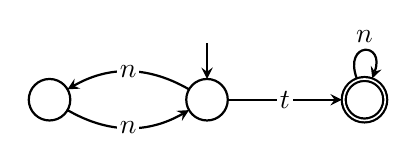
\begin{tikzpicture}[
                        > = stealth,
                        thick,
                        node distance = 2cm,
                        % font = \footnotesize
                    ]
                        \node[state, initial above] (0) {};
                        \node[state] (1) [left of = 0] {};
                        \node[state, accepting] (2) [right of = 0]{};
                
                        \path[->] (0) edge[bend right] node {$n$} (1);    
                        \path[->] (0) edge node {$t$} (2); 
                        \path[->] (1) edge[bend right] node {$n$} (0);
                        \path[->] (2) edge[loop above] node {$n$} (2);
                    \end{tikzpicture}
                }
                \subcaption{\color{teal} \scriptsize recognizes $\displaystyle \bigcup_{k \in \bb{N}} n^{2k} t n^*$}
            \end{subfigure}%
            \begin{subfigure}{0.5\linewidth}
                \centering
                \scalebox{0.75}{
                    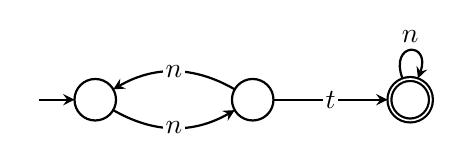
\begin{tikzpicture}[
                        > = stealth,
                        thick,
                        node distance = 2cm,
                        % font = \footnotesize
                    ]
                        \node[state] (0) {};
                        \node[state, initial] (1) [left of = 0] {};
                        \node[state, accepting] (2) [right of = 0]{};
                
                        \path[->] (0) edge[bend right] node {$n$} (1);    
                        \path[->] (0) edge node {$t$} (2); 
                        \path[->] (1) edge[bend right] node {$n$} (0);
                        \path[->] (2) edge[loop above] node {$n$} (2);
                    \end{tikzpicture}
                }
                \subcaption{\color{teal} \scriptsize recognizes $\displaystyle \bigcup_{k \in \bb{N}} n^{2k+1} t n^*$}
            \end{subfigure}
        \end{figure}
    \end{frame}

    

    \begin{frame}{Deep Reinforcement Learning}

        % Approximate policies $\pi : \tsc{states} \to \tsc{actions}$ in two stages:
        % \begin{enumerate}
        %     \item \teal{representation},
        %     \item \teal{(neural) interpretation}.
        % \end{enumerate}

        % \teal{\bf Traditional Approach:} uses feed-forward neural networks to interpret numerical state representations.

        Traditionally, a policy $\pi$ is approximated by a neural network $N$.

        % \begin{equation*}
        %     \pi : \textrm{States} \to \textrm{Actions} \qquad \approx \qquad N : \textrm{FeatureVectors} \to \textrm{Actions}
        % \end{equation*}

        \vspace{3ex}

            \begin{center}
                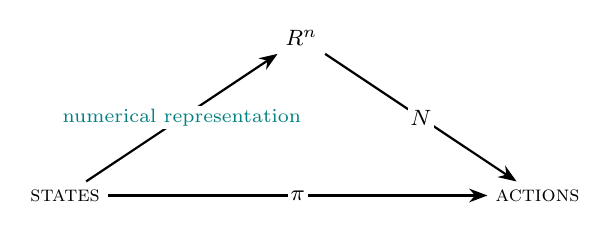
\begin{tikzpicture}[font = \footnotesize]
                    % \draw[step = 1cm, lightgray, very thin] (-3, -3) grid (3, 3);
                    \node (s) at (-3, 0) {\tsc{states}};
                    \node (a) at (3, 0) {\tsc{actions}};
                    \node (r) at (0, 2) {$\bb{R}^n$};
                    % \node (b) at (0, -1.5) {$2^{\Sigma^*}$};

                    \graph{
                        (r) <-["\scriptsize \teal{numerical representation}"] (s) ->["$\pi$"] (a),
                        (r) ->["$N$"] (a)
                        % (s) ->[blue] (b) ->[dashed, "?"] (a)
                    };
                \end{tikzpicture}
            \end{center}
        \end{frame}
            
\begin{frame}{Symbolic Deep Reinforcement Learning}         
    \begin{center}
                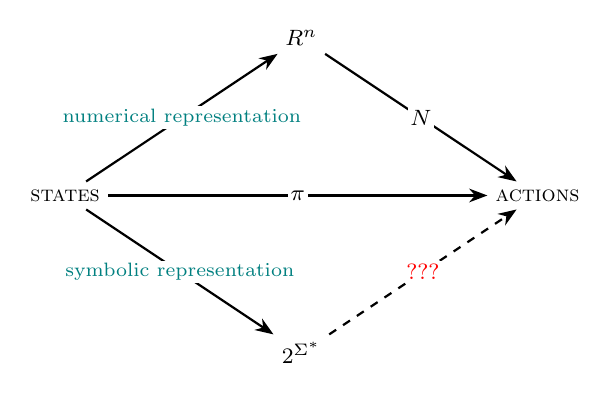
\begin{tikzpicture}[font = \footnotesize]
                    % \draw[step = 1cm, lightgray, very thin] (-3, -3) grid (3, 3);
                    \node (s) at (-3, 0) {\tsc{states}};
                    \node (a) at (3, 0) {\tsc{actions}};
                    \node (r) at (0, 2) {$\bb{R}^n$};
                    \node (b) at (0, -2) {$2^{\Sigma^*}$};

                    \graph{
                        (r) <-["\scriptsize \teal{numerical representation}"] (s) ->["$\pi$"] (a),
                        (r) ->["$N$"] (a),
                        (s) ->["\scriptsize \teal{symbolic representation}"] (b) ->[dashed, "\red{???}"] (a)
                    };
                \end{tikzpicture}
            \end{center}

            Can the deep RL approach be adapted around \teal{symbolic representation} of states as formal languages?
    \end{frame}

    \begin{frame}{Deep Regular Reinforcement Learning}

        \begin{center}
            \begin{tikzpicture}[font = \footnotesize]
                % \draw[step = 1cm, lightgray, very thin] (-3, -3) grid (3, 3);
                \node (s) at (-3, 0) {\tsc{states}};
                \node (a) at (3, 0) {\tsc{actions}};
                \node (r) at (0, 2) {$\bb{R}^n$};
                \node (b) at (0, -2) {$2^{\Sigma^*}$};

                \graph{
                    (r) <-["\scriptsize numerical representation"] (s) ->["$\pi$"] (a),
                    (r) ->["$N$"] (a),
                    (s) ->["\teal{\bf regular}\\\scriptsize symbolic representation"] (b) ->["$G$"] (a)
                };

                \node[label = {[name = aut]:\teal{\scriptsize automaton}}] (A) at (-3, -4.5) {\includegraphics[scale = 0.75]{~/Documents/projects/dissertation/figures/main-figure11.pdf}\quad};

                \node[label = \teal{\scriptsize action}, rounded corners, inner sep = 5pt] (aa) at (4, -4.5) {$a$};

                \path[->] (A) edge node[label = \teal{\scriptsize graph neural network}] {$G$} (aa);

                \node[fit = (a)(b), draw = blue, thin, rounded corners, fill opacity = 0, rotate = 33, inner ysep = -22pt, inner xsep = 10pt, yshift = 2pt] (g) {};

                \node[fit = (A)(aa)(aut), draw = blue, thin, rounded corners, fill opacity = 0, inner sep = 5pt] (z) {};

                \path[-] (g.south) edge[blue, bend left, thin] (z);
            \end{tikzpicture}
        \end{center}

        

        % \teal{\bf Deep Regular RL:} approximate a policy $\pi$ with a graph neural network $G$ via symbolic representation.

            % \begin{equation*}
            %     \pi : \textrm{States} \to \textrm{Actions} \qquad \approx \qquad G : \textrm{FiniteAutomata} \to \textrm{Actions}
            % \end{equation*}

        % \begin{block}{Deep RL}
        %     \footnotesize A policy is approximated by a \emph{\teal{\textrm{neural network}}}
        %     \begin{equation*}
        %         \pi : \textrm{States} \to \textrm{Actions} \qquad \approx \qquad N : \textrm{FeatureVectors} \to \textrm{Actions}.
        %     \end{equation*}
        % \end{block}

        % \begin{block}{Deep \textit{Regular} RL}
        %     \footnotesize A policy is approximated by a \emph{\teal{\textrm{graph neural network}}}
        %     \begin{equation*}
        %         \pi : \textrm{States} \to \textrm{Actions} \qquad \approx \qquad G : \textrm{FiniteAutomata} \to \textrm{Actions}.
        %     \end{equation*}
        % \end{block}
        % \pause

        % \vspace{3ex}

        % \begin{center}
        %     % \vspace{1ex}
        %     % \resizebox{\textwidth}{!}{
        %     \tcbox[colback=white, colframe=teal!75!black]{
        %         \begin{tikzpicture}
        %             \node[label = \teal{\scriptsize automaton}] (A) at (0, 0) {\includegraphics[scale = 0.75]{~/Documents/projects/dissertation/figures/main-figure11.pdf}\quad};

        %             \node[label = \teal{\scriptsize action}, rounded corners, inner sep = 5pt] (a) at (7, 0) {$a$};

        %             \path[->] (A) edge node[label = \teal{\scriptsize graph neural network}] {$G$} (a);

        %             \node[fit=]
        %         \end{tikzpicture}
        %     } 
        % \end{center}
    \end{frame}

    \begin{frame}{Deep Regular Reinforcement Learning --- Modified Tangrams}
        \begin{overprint}
            \onslide<1>
            \begin{figure}[t!]
                \vspace{3ex}
                \begin{subfigure}[T]{0.475\linewidth}
                    \centering
                    \includegraphics[width = \linewidth]{~/Documents/projects/dissertation/figures/main-figure28.pdf}
                    \subcaption{initial configuration}
                \end{subfigure}
                \hfill
                \begin{subfigure}[T]{0.475\linewidth}
                    \centering
                    \includegraphics[width = \linewidth]{~/Documents/projects/dissertation/figures/main-figure29.pdf}
                    \subcaption{solution}
                \end{subfigure}
            \end{figure}

            \onslide<2>            
            % {\footnotesize
                For any $b \in \bb{N}$, each $w \in \set{0, ... , b-1}^*$ encodes an element of $[0, 1]$ as
                \begin{equation*}
                    w_b = \sum^{\card{w}}_{k=1} \frac{w(k)}{b^k}.
                \end{equation*}
            % }        
    
            % \vspace{-5ex}

            \begin{figure}
                \centering
                \resizebox{0.8\linewidth}{!}{
                    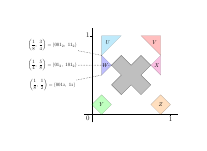
\begin{tikzpicture}[ultra thin]

                        \path (-0.1, 0) edge (1.1, 0);
                        \path (0, -0.1) edge (0, 1.1);
                        \node[inner sep = 0pt, outer sep = 0pt, scale=0.25] (y) at (-0.05, 1) {\rm 1};
                        \path (y) edge (0, 1);
                        \node[inner sep = 0pt, outer sep = 1pt, scale=0.25] (x) at (1, -0.06) {\rm 1};
                        \path (x.north) edge (1, 0);
                        \node[scale = 0.25] at (-0.05, -0.05) {\rm 0};

                        \filldraw[gray, opacity = 0.5, draw = black] (1/2, 5/8) -- (5/8, 3/4) -- (3/4, 5/8) -- (5/8, 1/2) -- (3/4, 3/8) -- (5/8, 1/4) -- (1/2, 3/8) -- (3/8, 1/4) -- (1/4, 3/8) -- (3/8, 1/2) -- (1/4, 5/8) -- (3/8, 3/4) -- (1/2, 5/8);
        
                        \filldraw[cyan, opacity = 0.25, draw = black] (1/8, 3/4) -- (1/8, 1) -- (3/8, 1) -- (1/8, 3/4);
                        \node[scale = 0.2, inner sep = 0pt, fill = none] at (13/64, 11/12) {$U$};
        
                        \filldraw[red, opacity = 0.25, draw = black] (7/8, 3/4) -- (7/8, 1) -- (5/8, 1) -- (7/8, 3/4);
                        \node[scale = 0.2, inner sep = 0pt, fill = none] at (51/64, 11/12) {$V$};

                        \filldraw[blue, opacity = 0.25, draw = black, ultra thin] (1/8, 3/4) -- (1/8, 1/2) -- (1/4, 5/8) -- (1/8, 3/4);
                        \node[scale = 0.2, inner sep = 0pt, fill = none] (W) at (11/64, 5/8) {$W$};

                        \node[scale = 0.2, fill = none] at (1/8, 3/4) {};
                        \node[scale = 0.2, fill = none] at (1/8, 1/2) {};
                        \node[scale = 0.2, fill = none] at (1/4, 5/8) {};

                        \node[scale = 0.175] (x) at (-0.5, 7/8) {$\displaystyle \paren*{\frac{1}{8},~ \frac{3}{4}} = \paren*{{001}_2,~ {11}_2}$};
                        \node[scale = 0.175] (y) at (-0.5, 3/8) {$\displaystyle \paren*{\frac{1}{8},~ \frac{1}{2}} = \paren*{{001}_2,~ {1}_2}$};
                        \node[scale = 0.175] (z) at (-0.5, 5/8) {$\displaystyle \paren*{\frac{1}{4},~ \frac{5}{8}} = \paren*{{01}_2,~ {101}_2}$};

                        \draw [very thin, dots=50 per 1cm] (1/8, 3/4) -- (x);
                        \draw [very thin, dots=50 per 1cm] (1/8, 1/2) -- (y);
                        \draw [very thin, dots=50 per 1cm] (1/4, 5/8) -- (z);

                        \filldraw[magenta, opacity = 0.25, draw = black] (7/8, 3/4) -- (7/8, 1/2) -- (3/4, 5/8) -- (7/8, 3/4);
                        \node[scale = 0.2, inner sep = 0pt, fill = none] at (53/64, 5/8) {$X$};
        
                        \filldraw[green, opacity = 0.25, draw = black] (0, 1/8) --  (1/8, 1/4) -- (1/4, 1/8) -- (1/8, 0) -- (0, 1/8);
                        \node[scale = 0.2, inner sep = 0pt, fill = none] at (1/8, 1/8) {$Y$};
        
                        \filldraw[orange, opacity = 0.25, draw = black] (1, 1/8) -- (7/8, 1/4) -- (3/4, 1/8) -- (7/8, 0) -- (1, 1/8);
                        \node[scale = 0.2, inner sep = 0pt, fill = none] at (7/8, 1/8) {$Z$};
                    \end{tikzpicture}
                }
            \end{figure}
            
            \onslide<3>
            \begin{figure}
                % \centering
                \resizebox{!}{0.5\textheight}{
                    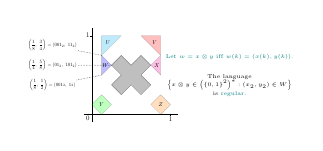
\begin{tikzpicture}[ultra thin]

                        \path (-0.1, 0) edge (1.1, 0);
                        \path (0, -0.1) edge (0, 1.1);
                        \node[inner sep = 0pt, outer sep = 0pt, scale=0.25] (y) at (-0.05, 1) {\rm 1};
                        \path (y) edge (0, 1);
                        \node[inner sep = 0pt, outer sep = 1pt, scale=0.25] (x) at (1, -0.06) {\rm 1};
                        \path (x.north) edge (1, 0);
                        \node[scale = 0.25] at (-0.05, -0.05) {\rm 0};

                        \filldraw[gray, opacity = 0.5, draw = black] (1/2, 5/8) -- (5/8, 3/4) -- (3/4, 5/8) -- (5/8, 1/2) -- (3/4, 3/8) -- (5/8, 1/4) -- (1/2, 3/8) -- (3/8, 1/4) -- (1/4, 3/8) -- (3/8, 1/2) -- (1/4, 5/8) -- (3/8, 3/4) -- (1/2, 5/8);
        
                        \filldraw[cyan, opacity = 0.25, draw = black] (1/8, 3/4) -- (1/8, 1) -- (3/8, 1) -- (1/8, 3/4);
                        \node[scale = 0.2, inner sep = 0pt, fill = none] at (13/64, 11/12) {$U$};
        
                        \filldraw[red, opacity = 0.25, draw = black] (7/8, 3/4) -- (7/8, 1) -- (5/8, 1) -- (7/8, 3/4);
                        \node[scale = 0.2, inner sep = 0pt, fill = none] at (51/64, 11/12) {$V$};

                        \filldraw[blue, opacity = 0.25, draw = black, ultra thin] (1/8, 3/4) -- (1/8, 1/2) -- (1/4, 5/8) -- (1/8, 3/4);
                        \node[scale = 0.2, inner sep = 0pt, fill = none] (W) at (11/64, 5/8) {$W$};

                        \node[scale = 0.2, fill = none] at (1/8, 3/4) {};
                        \node[scale = 0.2, fill = none] at (1/8, 1/2) {};
                        \node[scale = 0.2, fill = none] at (1/4, 5/8) {};

                        \node[scale = 0.175] (x) at (-0.5, 7/8) {$\displaystyle \paren*{\frac{1}{8},~ \frac{3}{4}} = \paren*{{001}_2,~ {11}_2}$};
                        \node[scale = 0.175] (y) at (-0.5, 3/8) {$\displaystyle \paren*{\frac{1}{8},~ \frac{1}{2}} = \paren*{{001}_2,~ {1}_2}$};
                        \node[scale = 0.175] (z) at (-0.5, 5/8) {$\displaystyle \paren*{\frac{1}{4},~ \frac{5}{8}} = \paren*{{01}_2,~ {101}_2}$};

                        \draw [very thin, dots=50 per 1cm] (1/8, 3/4) -- (x);
                        \draw [very thin, dots=50 per 1cm] (1/8, 1/2) -- (y);
                        \draw [very thin, dots=50 per 1cm] (1/4, 5/8) -- (z);

                        \filldraw[magenta, opacity = 0.25, draw = black] (7/8, 3/4) -- (7/8, 1/2) -- (3/4, 5/8) -- (7/8, 3/4);
                        \node[scale = 0.2, inner sep = 0pt, fill = none] at (53/64, 5/8) {$X$};
        
                        \filldraw[green, opacity = 0.25, draw = black] (0, 1/8) --  (1/8, 1/4) -- (1/4, 1/8) -- (1/8, 0) -- (0, 1/8);
                        \node[scale = 0.2, inner sep = 0pt, fill = none] at (1/8, 1/8) {$Y$};
        
                        \filldraw[orange, opacity = 0.25, draw = black] (1, 1/8) -- (7/8, 1/4) -- (3/4, 1/8) -- (7/8, 0) -- (1, 1/8);
                        \node[scale = 0.2, inner sep = 0pt, fill = none] at (7/8, 1/8) {$Z$};

                        \node[align = center, font = \tiny, scale = 0.4] at (1.75, 0.5) {
                            \teal{Let $w = x \otimes y$ iff $w(k) = (x(k), y(k))$.} \\
                            \\
                            \\
                            The language \\
                            $\displaystyle \set*{x \otimes y \in \paren*{\set*{0, 1}^2}^* : \paren*{x_2, y_2} \in W}$ \\
                            is \teal{regular}.
                        };
                    \end{tikzpicture}
                }
            \end{figure}
            \vspace*{-5ex}
            \begin{figure}
                \centering
                % \includegraphics[width = \linewidth]{~/Documents/projects/dissertation/figures/main-figure32.pdf}
                \resizebox{!}{0.5\textheight}{
                    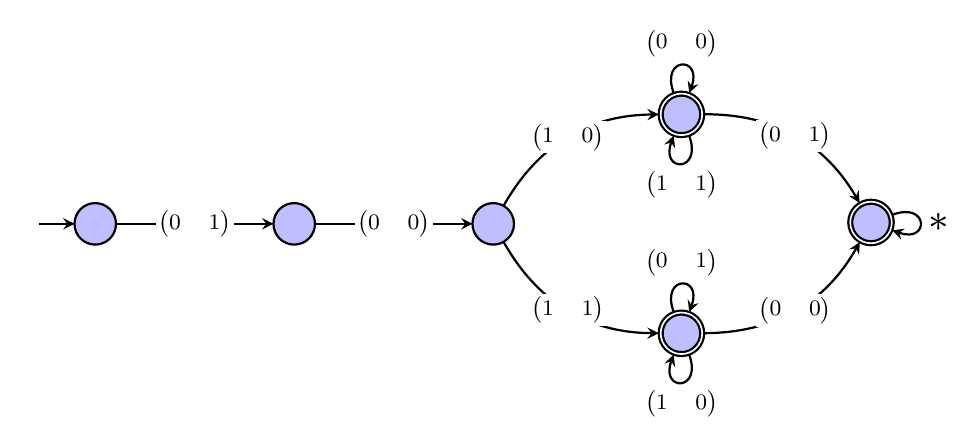
\begin{tikzpicture}[>= stealth, node distance = 2cm, node font = \footnotesize]
                        \node[state, initial, fill = blue!25] (0) {};
                        \node[state, fill = blue!25] [right = 2cm of 0] (1) {};
                        \node[state, fill = blue!25] [right = 2cm of 1] (2) {};
                        \node[state, accepting, fill = blue!25] [above right = 1cm and 2cm of 2] (3) {};
                        \node[state, accepting, fill = blue!25] [below right = 1cm and 2cm of 2] (4) {};
                        \node[state, accepting, fill = blue!25] [above right = 1cm and 2cm of 4] (5) {};
        
                        \path[->] (0) edge node {$\begin{pmatrix} 0 & 1 \end{pmatrix}$} (1);
                        \path[->] (1) edge node {$\begin{pmatrix} 0 & 0 \end{pmatrix}$} (2);
                        \path[->] (2) edge[bend left] node {$\begin{pmatrix} 1 & 0 \end{pmatrix}$} (3);
                        \path[->] (2) edge[bend right] node {$\begin{pmatrix} 1 & 1 \end{pmatrix}$} (4);
                        \path[->] (3) edge[bend left] node {$\begin{pmatrix} 0 & 1 \end{pmatrix}$} (5);
                        \path[->] (4) edge[bend right] node {$\begin{pmatrix} 0 & 0 \end{pmatrix}$} (5);
                        \path[->] (3) edge[loop above] node {$\begin{pmatrix} 0 & 0 \end{pmatrix}$} (3);
                        \path[->] (3) edge[loop below] node {$\begin{pmatrix} 1 & 1 \end{pmatrix}$} (3);
                        \path[->] (4) edge[loop above] node {$\begin{pmatrix} 0 & 1 \end{pmatrix}$} (4);
                        \path[->] (4) edge[loop below] node {$\begin{pmatrix} 1 & 0 \end{pmatrix}$} (4);
                        \path[->] (5) edge[loop right] node {$\bigast$} (5);
                    \end{tikzpicture}
                }
                % \subcaption{\color{teal}\scriptsize automaton representation of $V$}
            \end{figure}

            \onslide<4>

            \vspace{0.5cm}
            \begin{figure}
                \begin{subfigure}[T]{0.45\linewidth}
                    \centering
                    \subcaption{\color{teal} translate right by $1/2$}
                    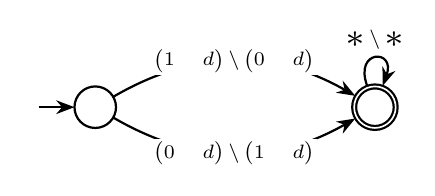
\begin{tikzpicture}[node font = {\scriptsize}]
                        \node[state, initial] (0) {};
                        \node[state, accepting] (1) [right = 3cm of 0] {};
                
                        \path[->] (0) edge[bend left] node {$\begin{pmatrix} 1 & d \end{pmatrix} \backslash \begin{pmatrix} 0 & d \end{pmatrix}$} (1);
                        \path[->] (0) edge[bend right] node {$\begin{pmatrix} 0 & d \end{pmatrix} \backslash \begin{pmatrix} 1 & d \end{pmatrix}$} (1);
            
                        \path[->] (1) edge[loop above] node {$\bigast \backslash \bigast$} (1);
                    \end{tikzpicture}
                \end{subfigure}%
                \begin{subfigure}[T]{0.45\linewidth}
                    \centering
                    \subcaption{\color{teal} reflect about $y = 1/2$}
                    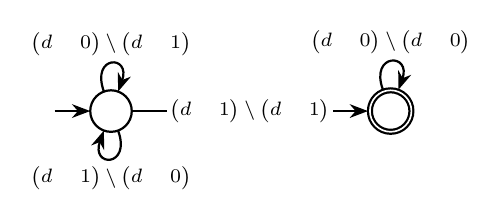
\begin{tikzpicture}[thick, node font = {\scriptsize}]
                        \node[state, initial] (0) {};
                        \node[state, accepting] (1) [right = 3cm of 0] {};
                        
                        \path[->] (0) edge[loop above] node {$\begin{pmatrix} d & 0 \end{pmatrix} \backslash \begin{pmatrix} d & 1 \end{pmatrix}$} (0);
                        \path[->] (0) edge[loop below] node {$\begin{pmatrix} d & 1 \end{pmatrix} \backslash \begin{pmatrix} d & 0 \end{pmatrix}$} (0);
                        \path[->] (0) edge node {$\begin{pmatrix} d & 1 \end{pmatrix} \backslash \begin{pmatrix} d & 1 \end{pmatrix}$} (1);
                        \path[->] (1) edge[loop above] node {$\begin{pmatrix} d & 0 \end{pmatrix} \backslash \begin{pmatrix} d & 0 \end{pmatrix}$} (1);
                    \end{tikzpicture}
                \end{subfigure}
                \caption{
                    \color{teal}
                    Transducers implementing rigid transformations on the unit square.
                }
                % \label{fig:tangram_transducers}
                % \vspace{-3ex}
            \end{figure}

            % \vspace{2ex}

            \tcbox[
                colback = white,
                colframe = teal
            ]{
               \footnotesize
               Can an RL agent effectively solve tangram-style puzzles modeled as RMDPs?
            }
            
            \vspace{5ex}

            \footnotetext{\scriptsize Digits $d$ are arbitrary but must match on each side of $\backslash$. $*$ represents arbitrary pairs of digits.}

            \onslide<5>
            \begin{figure}
                \hspace{-20pt}
                \centering
                \includegraphics[scale = 0.95]{~/Documents/projects/dissertation/figures/main-figure36.pdf}
            \end{figure}
        \end{overprint}

        % \note{
        %     \begin{itemize}
        %         \item
        %             * is shorthand for arbitrary pairs
        %         \item
        %             $d$ represents an arbitrary binary symbol
        %         \item
        %             An annotated reward curve for the modified tangram example.
        %             The dark line shows the mean, and the shaded region shows the $10^{th}$ and $90^{th}$ percentiles over $5$ training runs.
        %             The four annotated parts of the curve show the agent's progress.
        %             We selected an arbitrary training run, and executed the policy of the agent at these points in the training run, and the final configurations produced by the agent are shown.
        %     \end{itemize}
        % }
    \end{frame}

    \begin{frame}{Further Experimental Studies}
        \vspace{-3ex}
        % \begin{columns}
            % \begin{column}{0.33\linewidth}
                \begin{figure}
                    % \vspace{-2ex}
                    % \begin{subfigure}[T]{0.24\linewidth}
                    %     \centering
                    %     \resizebox{\linewidth}{!}{%
                    %         \begin{tabular}{c|c}
                    %             State \:&\: Action \\
                    %             \hline
                    %             3*3+7+5\#\# \:&\: Move \\
                    %             *3+7+5\#\#3 \:&\: Push \\
                    %             3+7+5\#*\#3 \:&\: Move \\
                    %             +7+5\#*\#33 \:&\: Pop \\
                    %             +7+5\#\#33* \:&\: Push \\
                    %             7+5\#+\#33* \:&\: Move \\
                    %             +5\#+\#33*7 \:&\: Pop \\
                    %             +5\#\#33*7+ \:&\: Push \\
                    %             5\#+\#33*7+ \:&\: Move \\
                    %             \#+\#33*7+5 \:&\: Pop \\
                    %             \#\#33*7+5+
                    %         \end{tabular}
                    %     }
                    % \end{subfigure}%
                    % % \hspace{1em}
                    % \begin{subfigure}[T]{0.24\linewidth}
                    %     \centering
                    %     \resizebox{\linewidth}{!}{%
                    %         \begin{tabular}{c|c}
                    %             State \:&\: Action \\
                    %             \hline
                    %             1+7*8+0\#\# \:&\: Move \\
                    %             +7*8+0\#\#1 \:&\: Push \\
                    %             7*8+0\#+\#1 \:&\: Move \\
                    %             *8+0\#+\#17 \:&\: Push \\
                    %             8+0\#+*\#17 \:&\: Move \\
                    %             +0\#+*\#178 \:&\: Pop \\
                    %             +0\#+\#178* \:&\: Pop \\
                    %             +0\#\#178*+ \:&\: Push \\
                    %             0\#+\#178*+ \:&\: Move \\
                    %             \#+\#178*+0 \:&\: Pop \\
                    %             \#\#178*+0+
                    %         \end{tabular}
                    %     }
                    % \end{subfigure}%
                    \begin{subfigure}[T]{0.25\linewidth}
                        \centering
                        \resizebox{\linewidth}{!}{%
                            \begin{tabular}{c|c}
                                State \:&\: Action \\
                                \hline
                                7-1*3\#\# \:&\: Move \\
                                -1*3\#\#7 \:&\: Push \\
                                1*3\#-\#7 \:&\: Move \\
                                *3\#-\#71 \:&\: Push \\
                                3\#-*\#71 \:&\: Move \\
                                \#-*\#713 \:&\: Pop \\
                                \#-\#713* \:&\: Pop \\
                                \#\#713*-
                            \end{tabular}
                        }
                    \end{subfigure}
                    \hspace{1cm}
                    \begin{subfigure}[T]{0.4\linewidth}
                        \includegraphics[width = \linewidth]{/home/taylor/Desktop/CAV_CameraReady_RRL/shunting_yard_algorithm.pdf}
                    \end{subfigure}
                    % \caption{Runs produced by the learned policy for the shunting yard algorithm.}
                    % \label{fig:shunting_traj}
                    % \vspace{-2ex}
                \end{figure}

                \vspace{-2ex}

                \begin{figure}
                    \begin{subfigure}{0.45\linewidth}
                        \resizebox{\linewidth}{!}{
                        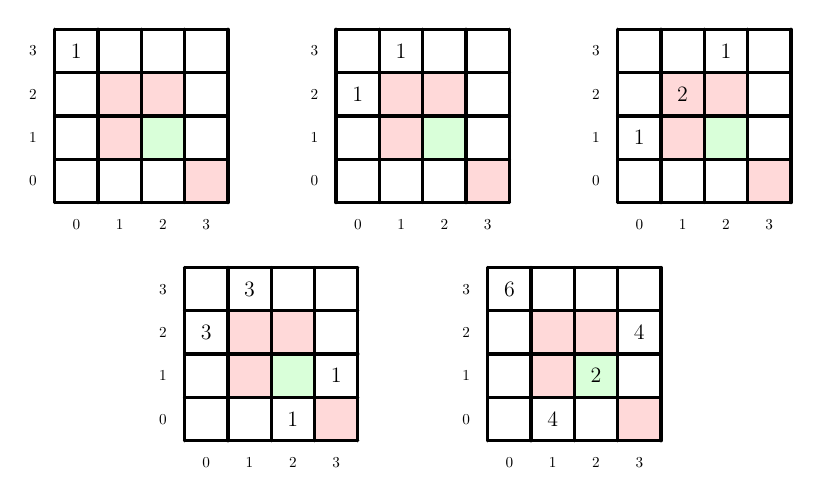
\begin{tikzpicture}[scale=0.55,transform shape]
                            \begin{scope}
                                \foreach \y in {0,...,3} {
                                    \path (0.5+\y,-0.5) node {$\y$};
                                    \path (-0.5,0.5+\y) node {$\y$};
                                }
                                \fill[red!15] (1,1) rectangle (2,2);
                                \fill[red!15] (1,2) rectangle (2,3);
                                \fill[green!15] (2,1) rectangle (3,2);
                                \fill[red!15] (2,2) rectangle (3,3);
                                \fill[red!15] (3,0) rectangle (4,1);
                                \path (0.5,3.5) node {\Large$1$};
                                \draw[very thick, cap=round] (0,0) grid (4,4);            
                            \end{scope}
                            \begin{scope}[xshift=6.5cm]
                                \foreach \y in {0,...,3} {
                                    \path (0.5+\y,-0.5) node {$\y$};
                                    \path (-0.5,0.5+\y) node {$\y$};
                                }
                                \fill[red!15] (1,1) rectangle (2,2);
                                \fill[red!15] (1,2) rectangle (2,3);
                                \fill[green!15] (2,1) rectangle (3,2);
                                \fill[red!15] (2,2) rectangle (3,3);
                                \fill[red!15] (3,0) rectangle (4,1);
                                \path (1.5,3.5) node {\Large$1$};
                                \path (0.5,2.5) node {\Large$1$};
                                \draw[very thick, cap=round] (0,0) grid (4,4);            
                            \end{scope}
                            \begin{scope}[xshift=13cm]
                                \foreach \y in {0,...,3} {
                                    \path (0.5+\y,-0.5) node {$\y$};
                                    \path (-0.5,0.5+\y) node {$\y$};
                                }
                                \fill[red!15] (1,1) rectangle (2,2);
                                \fill[red!15] (1,2) rectangle (2,3);
                                \fill[green!15] (2,1) rectangle (3,2);
                                \fill[red!15] (2,2) rectangle (3,3);
                                \fill[red!15] (3,0) rectangle (4,1);
                                \path (2.5,3.5) node {\Large$1$};
                                \path (0.5,1.5) node {\Large$1$};
                                \path (1.5,2.5) node [fill=red!15] {\Large$2$};
                                \draw[very thick, cap=round] (0,0) grid (4,4);            
                            \end{scope}
                            \begin{scope}[yshift=-5.5cm, xshift=3cm]
                                \foreach \y in {0,...,3} {
                                    \path (0.5+\y,-0.5) node {$\y$};
                                    \path (-0.5,0.5+\y) node {$\y$};
                                }
                                \fill[red!15] (1,1) rectangle (2,2);
                                \fill[red!15] (1,2) rectangle (2,3);
                                \fill[green!15] (2,1) rectangle (3,2);
                                \fill[red!15] (2,2) rectangle (3,3);
                                \fill[red!15] (3,0) rectangle (4,1);
                                \path (1.5,3.5) node {\Large$3$};
                                \path (0.5,2.5) node {\Large$3$};
                                \path (2.5,0.5) node {\Large$1$};
                                \path (3.5,1.5) node {\Large$1$};
                                \draw[very thick, cap=round] (0,0) grid (4,4);            
                            \end{scope}
                            \begin{scope}[yshift=-5.5cm, xshift=10cm]
                                \foreach \y in {0,...,3} {
                                    \path (0.5+\y,-0.5) node {$\y$};
                                    \path (-0.5,0.5+\y) node {$\y$};
                                }
                                \fill[red!15] (1,1) rectangle (2,2);
                                \fill[red!15] (1,2) rectangle (2,3);
                                \fill[green!15] (2,1) rectangle (3,2);
                                \fill[red!15] (2,2) rectangle (3,3);
                                \fill[red!15] (3,0) rectangle (4,1);
                                \path (0.5,3.5) node {\Large$6$};
                                \path (2.5,1.5) node [fill=green!15] {\Large$2$};
                                \path (1.5,0.5) node {\Large$4$};
                                \path (3.5,2.5) node {\Large$4$};
                                \draw[very thick, cap=round] (0,0) grid (4,4); 
                            \end{scope}
                        \end{tikzpicture}
                    }
                        % \caption{
                        %     \scriptsize Execution of the optimal policy for the duplicating pebbles case study.
                        % }
                    \end{subfigure}
                    \begin{subfigure}{0.4\linewidth}
                        \includegraphics[width = \linewidth]{/home/taylor/Desktop/CAV_CameraReady_RRL/duplicating_pebbles.pdf}
                    \end{subfigure}
                \end{figure}
            % \end{column}
        % \end{columns}
    \end{frame}

    % \begin{frame}{Key Takeaways}
        
    % \end{frame}

    \begin{frame}
        \begin{center}
            \textbf{\teal{Questions?}}
        \end{center}
    \end{frame}

    % \tikzexternaldisable
    % \bibliographystyle{abbrvnat}
    % \nocite{*}
    % {\tiny\bibliography{references.bib}}

\end{document}